\documentclass[a4paper, 12pt, oneside]{article}
\usepackage[utf8]{inputenc}
\usepackage[margin=3cm, bindingoffset=1cm]{geometry}
\linespread{1.5}
\usepackage{float}
\usepackage{csquotes}
\usepackage{subfig}
\usepackage{graphicx}
\usepackage{indentfirst}
\usepackage{fancyhdr}
\usepackage{alphabeta}
\usepackage{algpseudocode}
\usepackage{algorithm}
\usepackage{hyperref}
\usepackage[T1]{fontenc}
\usepackage{listings}
\usepackage[htt]{hyphenat}
\usepackage{pgfplots}

\usepackage[
    backend=biber,
    sorting=none
]{biblatex}
\addbibresource{bibliography.bib}


\setlength{\parindent}{1cm}

\pagestyle{fancy}
\fancyhf{}
\fancyhead[C]{\textbf{\leftmark}}
\fancyfoot[C]{\thepage}
\renewcommand{\headrulewidth}{1pt}
\renewcommand{\footrulewidth}{1pt}
\renewcommand{\contentsname}{Indice}
\usepackage{caption}
\captionsetup[figure]{labelformat=empty}

\usepackage[Conny]{fncychap}

  
\begin{document}
\begin{titlepage}
    \begin{center}
        \LARGE{\uppercase{Università degli Studi di Salerno}}\\
        \vspace{5mm}
    	\uppercase{\normalsize Dipartimento di Informatica }\\
    \end{center}
    \begin{figure}[H]
        \centering
        
\includegraphics[width=0.35\textwidth]{logo_unisa}
    \end{figure}
    
    \begin{center}
        \normalsize{\textbf{Corso di Laurea Magistrale in Informatica}}\\
    	\vspace{10mm}
    	\LARGE{\textbf{Securing \textsc{MAVLink} protocol: a Post Quantum cryptography-based approach}}\\
    	\vspace{3mm}
        \large{\uppercase{Anno Accademico 2022/2023}}
    \end{center}

    \vspace{60mm}
    \noindent
    \begin{minipage}[t]{0.4\textwidth}
    	Relatore:\\\textbf{Prof.\\Arcangelo Castiglione}
    	\vspace{12mm}\\
    \end{minipage}
    \hfill
    \begin{minipage}[t]{0.4\textwidth}\raggedleft
    	Candidato: \\\textbf{Hermann Senatore}
    \end{minipage}
\end{titlepage}

\tableofcontents
\newpage

\begin{abstract}
    L'evoluzione tecnologica a cui si sta assistendo negli ultimi anni sta rivoluzionando pesantemente il mondo dell'aviazione, merito anche (e soprattutto) dei cosiddetti \textbf{UAV} (unmanned aerial vehicle), che comunemente vengono definiti \textbf{droni}, impiegati sia in contesto "civile" che in contesto militare. La potenziale delicatezza delle missioni che questi veicoli si trovano ad affrontare suggerisce dunque la necessità di definire dei requisiti di sicurezza che ne permettano un impiego più agevole. L'innovazione tecnologica porta però a nuove sfide anche nel campo della sicurezza. In particolare, i recenti progressi nel campo del \textbf{quantum computing} apre nuove sfide nel contesto della crittografia, rendendo quindi necessario sviluppare nuove tecniche resistenti ad attacchi veicolati mediante computer quantistici. In questo lavoro viene presentato un \textbf{proof of concept} di un'architettura basata principalmente sul protocollo MAVLink che permetta una comunicazione sicura tra un drone e la sua \textbf{Ground Control Station} e, ad un livello più alto, la definizione della chiave di cifratura utilizzata mediante il \textbf{Key Exchange Mechanism} Kyber, selezionato dal \textbf{NIST} come lo standard per quanto riguarda gli algoritmi di incapsulamento \textbf{quantum resistant}.
\end{abstract}
\newpage

\section{Introduzione}

\subsection{Scopi e struttura della tesi}
Il presente lavoro si concentra, come tra l'altro già accennato in precedenza nell'abstract, sull'analisi del proof of concept di un'architettura basata sul protocollo MAVLink che permetta lo scambio di chiavi e la comunicazione cifrata tra un UAV e la sua centrale di comando a terra utilizzando il KEM quantum-resistant Kyber e l'algoritmo AES in modo tale da proteggere lo scambio di messaggi tra i due \textit{endpoint} della comunicazione.

In particolare:

\begin{itemize}
    \item Questo capitolo funge da introduzione al lavoro svolto durante l'attività di Tesi, ne illustra la struttura e ne chiarisce le motivazioni ed il contesto in cui è calato;
    \item il \textbf{Capitolo 2} fornisce una panoramica sulle principali piattaforme software considerate nel presente lavoro;
    \item il \textbf{Capitolo 3} fornisce un'introduzione all'impatto dell'avvento dei \textbf{Computer Quantistici} nel campo della crittografia e al concetto di \textbf{Post-Quantum Cryptography} (PQC). Si procederà quindi ad una panoramica dell'algoritmo \textbf{Kyber};
    \item il \textbf{Capitolo 4} illustra in dettaglio le \textbf{modifiche} effettuate alle piattaforme software considerate nel presente lavoro ed al protocollo MAVLink stesso;
    \item il \textbf{Capitolo 5} fornisce le \textbf{conclusioni} al presente lavoro e illustra alcuni possibili \textbf{sviluppi futuri}.
\end{itemize}

\newpage


\subsection{UAV, APR o Droni: nomenclatura}
Nell'ultimo decennio, l'importante evoluzione tecnologica nel contesto dell'aviazione ha permesso la progettazione e la concreta realizzazione di veicoli in grado di volare e compiere missioni anche \textbf{senza la presenza di un pilota umano} sempre più versatili, efficaci e precisi. Questa tipologia di veicoli viene definita, a seconda del contesto linguistico in cui ci si trova, \textbf{UAV} (\textit{unmanned aerial vehicle}), \textbf{APR} (\textit{aeromobile a pilotaggio remoto}) o, più comunemente, \textbf{Drone}. Tutti questi acronimi sono, quindi, equivalenti tra di loro. 

La presenza di un essere umano continua tuttavia ad essere fondamentale in quanto il pilotaggio di questi dispositivi viene effettuato mentre una struttura di controllo "a terra", che prende il nome di \textbf{Ground Control Station} (da qui in poi \textit{GCS}). Tipicamente, una GCS può essere rappresentata da un qualsiasi apparato in grado di comunicare in qualche modo con l'UAV, quindi anche un comune Personal Computer su cui viene posto in esecuzione un software specifico.

\subsection{Cenni storici}
Il concetto di aeromobile senza pilota in sé non è sorprendentemente prerogativa degli ultimi anni e delle conseguenze che l'avvento delle tecnologie informatiche si porta dietro. Risale infatti agli Anni '40 del XIX secolo il primo (rudimentale!) impiego di "dispositivi" volanti senza pilota in campo militare. 

Per fronteggiare i moti rivoluzionari, peraltro diffusi anche in tutta Europa nel 1848, nella città di Venezia (che avevano portato alla creazione della cosiddetta Repubblica di San Marco), l'esercito austriaco lanciò dei \textbf{palloni} a cui era stato fissato dell'\textbf{esplosivo} dalla nave "Vulcano". 

Questo primo esperimento portò a risultati "misti": alcuni di questi dispositivi riuscirono effettivamente a colpire la città, altri furono invece deviati dal vento.

Per tutto il XIX secolo, lo sviluppo di questo tipo di dispositivi rimase prerogativa militare, con gli americani e gli inglesi che si occuparono dello sviluppo dei primi aeromobili comandati tramite radiofrequenza. Questi ultimi, nel 1917, testarono con successo un velivolo chiamato \textbf{Aerial Target}, mentre gli americani misero a punto il cosiddetto \textbf{Kettering Bug} \cite{drones-history}.

Nessuno di questi due prototipi venne tuttavia impiegato nella \textbf{prima guerra mondiale}.

Come già accennato in precedenza, con il passare del tempo e con il sempre più spinto progresso tecnologico i droni e, più in generale i veicoli a guida remota, hanno trovato un fertile campo di applicazione anche nell'ambito \textbf{civile}. Ad esempio, nel 2022 è stato proposto uno studio in cui è stato utilizzato un insieme di veicoli senza pilota per monitorare il processo di realizzazione di un \textbf{ponte} \cite{rs14081858}.
Si è assistito, riassumendo, ad una "democratizzazione" dell'uso dei droni negli ambiti più disparati.

\subsection{Sviluppi recenti}
Proprio questa diffusione più capillare dell'uso di suddetti veicoli a guida remota ha portato ad una più grande attenzione nello sviluppo di tecnologie software specifiche a questo ambito. 

A partire dagli anni 10 del XXI secolo sono stati concepiti diversi progetti software \textbf{open source} che forniscono piattaforme integrate compatibili con diversi tipi di apparati sia lato UAV che lato GCS. 

Parimenti, è stato necessario definire uno \textit{standard} per quanto riguarda l'ambito dei protocolli di comunicazione tra il drone e la sua \textit{GCS}, che è rappresentato sicuramente dal protocollo \textbf{MAVLink} e dalle sue successive evoluzioni. 

Una panoramica più approfondita sul protocollo MAVLink verrà in ogni caso affrontata nelle prossime sezioni in cui verranno illustrate le piattaforme software utilizzate nell'ambito del presente lavoro.

\newpage

\section{Piattaforme software per UAV e GCS}
Il presente capitolo fornisce una panoramica delle principali tecnologie utilizzate in ambito \textbf{civile} ed \textbf{amatoriale} nel contesto dei velivoli a pilotaggio remoto. In particolare viene riservata particolare attenzione ai seguenti due progetti \textbf{open source}:

\begin{itemize}
    \item \textbf{ArduPilot}: una piattaforma integrata scritta in \textbf{C++} utilizzabile su diverse tipologie di veicoli non necessariamente adatti al volo;
    \item \textbf{QGroundControl}: una \textbf{Ground Control Station} open source scritta in C++, che utilizza il framework \textbf{Qt} e che permette una più stretta interazione con la piattaforma ArduPilot.
\end{itemize}

\begin{figure}[H]
    \centering
    
\includegraphics[width=0.8\textwidth]{images/ardupilot_logo.png}
    \caption{Il logo di ArduPilot}
\end{figure}
\begin{figure}[H]
    \centering
    
\includegraphics[width=0.8\textwidth]{images/QGC_RGB_Logo_Horizontal_Positive_PREFERRED.png}
    \caption{Il logo di QGroundControl}
\end{figure}

Viene quindi svolta una panoramica sul protocollo di comunicazione \textbf{MAVLink} che permette l'interazione tra queste due componenti.

\begin{figure}[H]
    \centering
    
\includegraphics[width=0.8\textwidth]{images/logo_mavlink_small.png}
    \caption{Il logo del protocollo MAVLink}
\end{figure}

\newpage

\subsection{ArduPilot}

ArduPilot, come accennato, è una suite software universale che permette il controllo di diversi veicoli \textbf{non necessariamente volanti} \cite{ardupilot} la cui nascita risale al 2007.  L'idea di una suite software quale ArduPilot è stata formalizzata presso la piattaforma \textbf{DIYDrones.com}, community dedicata agli UAV fondata da \textbf{Chris Anderson} e che si definisce quindi "The Birthplace of ArduPilot"\cite{diy-drones}.

Nel 2009 venne prodotta la prima \textbf{board} che utilizzava questa piattaforma e nel novembre dello stesso anno il codice sorgente del progetto venne reso pubblico (ed è attualmente disponibile su GitHub all'url \url{https://github.com/ArduPilot/ardupilot})\cite{ardupilot-history}.

Correntemente, il progetto permette l'utilizzo su diverse tipologie di dispositivi, mediante delle versioni del firmware leggermente diverse tra di loro. In particolare, ArduPilot supporta dispositivi del tipo:

\begin{itemize}
    \item \textbf{Copter}: probabilmente quello più diffuso tra tutti e che tipicamente è composto da una board a cui sono associate diverse \textbf{eliche}. Il progetto di riferimento si chiama \textbf{ArduCopter}\cite{arducopter};
    \item \textbf{Plane}: un tipo di dispositivo ad \textbf{ala fissa}, tipicamente un \textbf{aereo radiocomandato}. Il progetto di riferimento si chiama \textbf{ArduPlane}\cite{arduplane};
    \item \textbf{Rover}: un tipo di dispositivo che non può spiccare il volo ma dotato di ruote e che di conseguenza viene utilizzato per missioni "a terra". Il progetto di riferimento si chiama semplicemente \textbf{Rover}\cite{rover};
    \item \textbf{Sub}: un tipo di dispositivo subacqueo, appartenente alla categoria degli \textbf{Autonomous Underwater Vehicles} (\textit{AUV}). Il progetto di riferimento si chiama \textbf{ArduSub}\cite{ardusub};
\end{itemize}

\begin{figure}[H]
    \centering
    \subfloat[\centering Copter]{{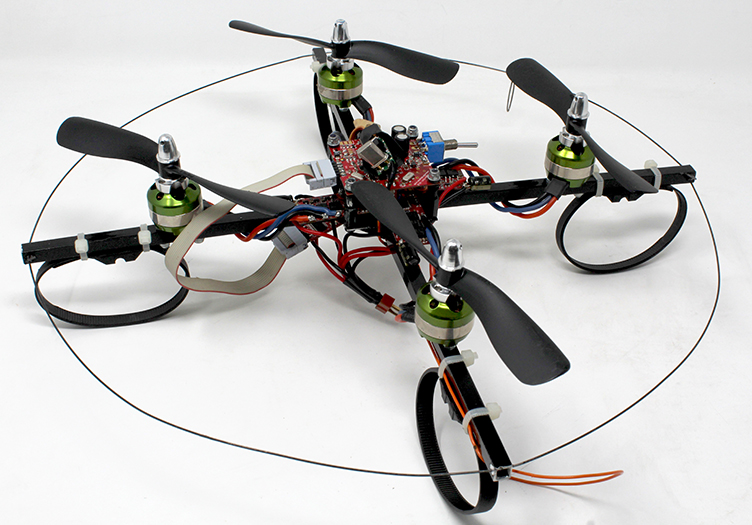
\includegraphics[width=0.4\textwidth]{images/copter.jpg} }}
    \qquad
    \subfloat[\centering Plane]{{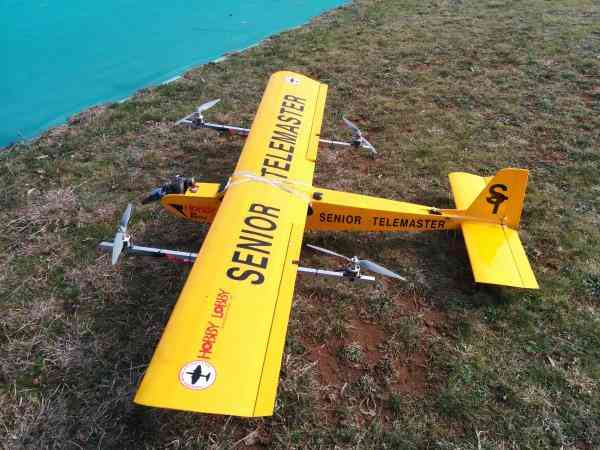
\includegraphics[width=0.4\textwidth]{images/plane.jpg} }}
\end{figure}
\begin{figure}[H]
    \centering
    \subfloat[\centering Rover]{{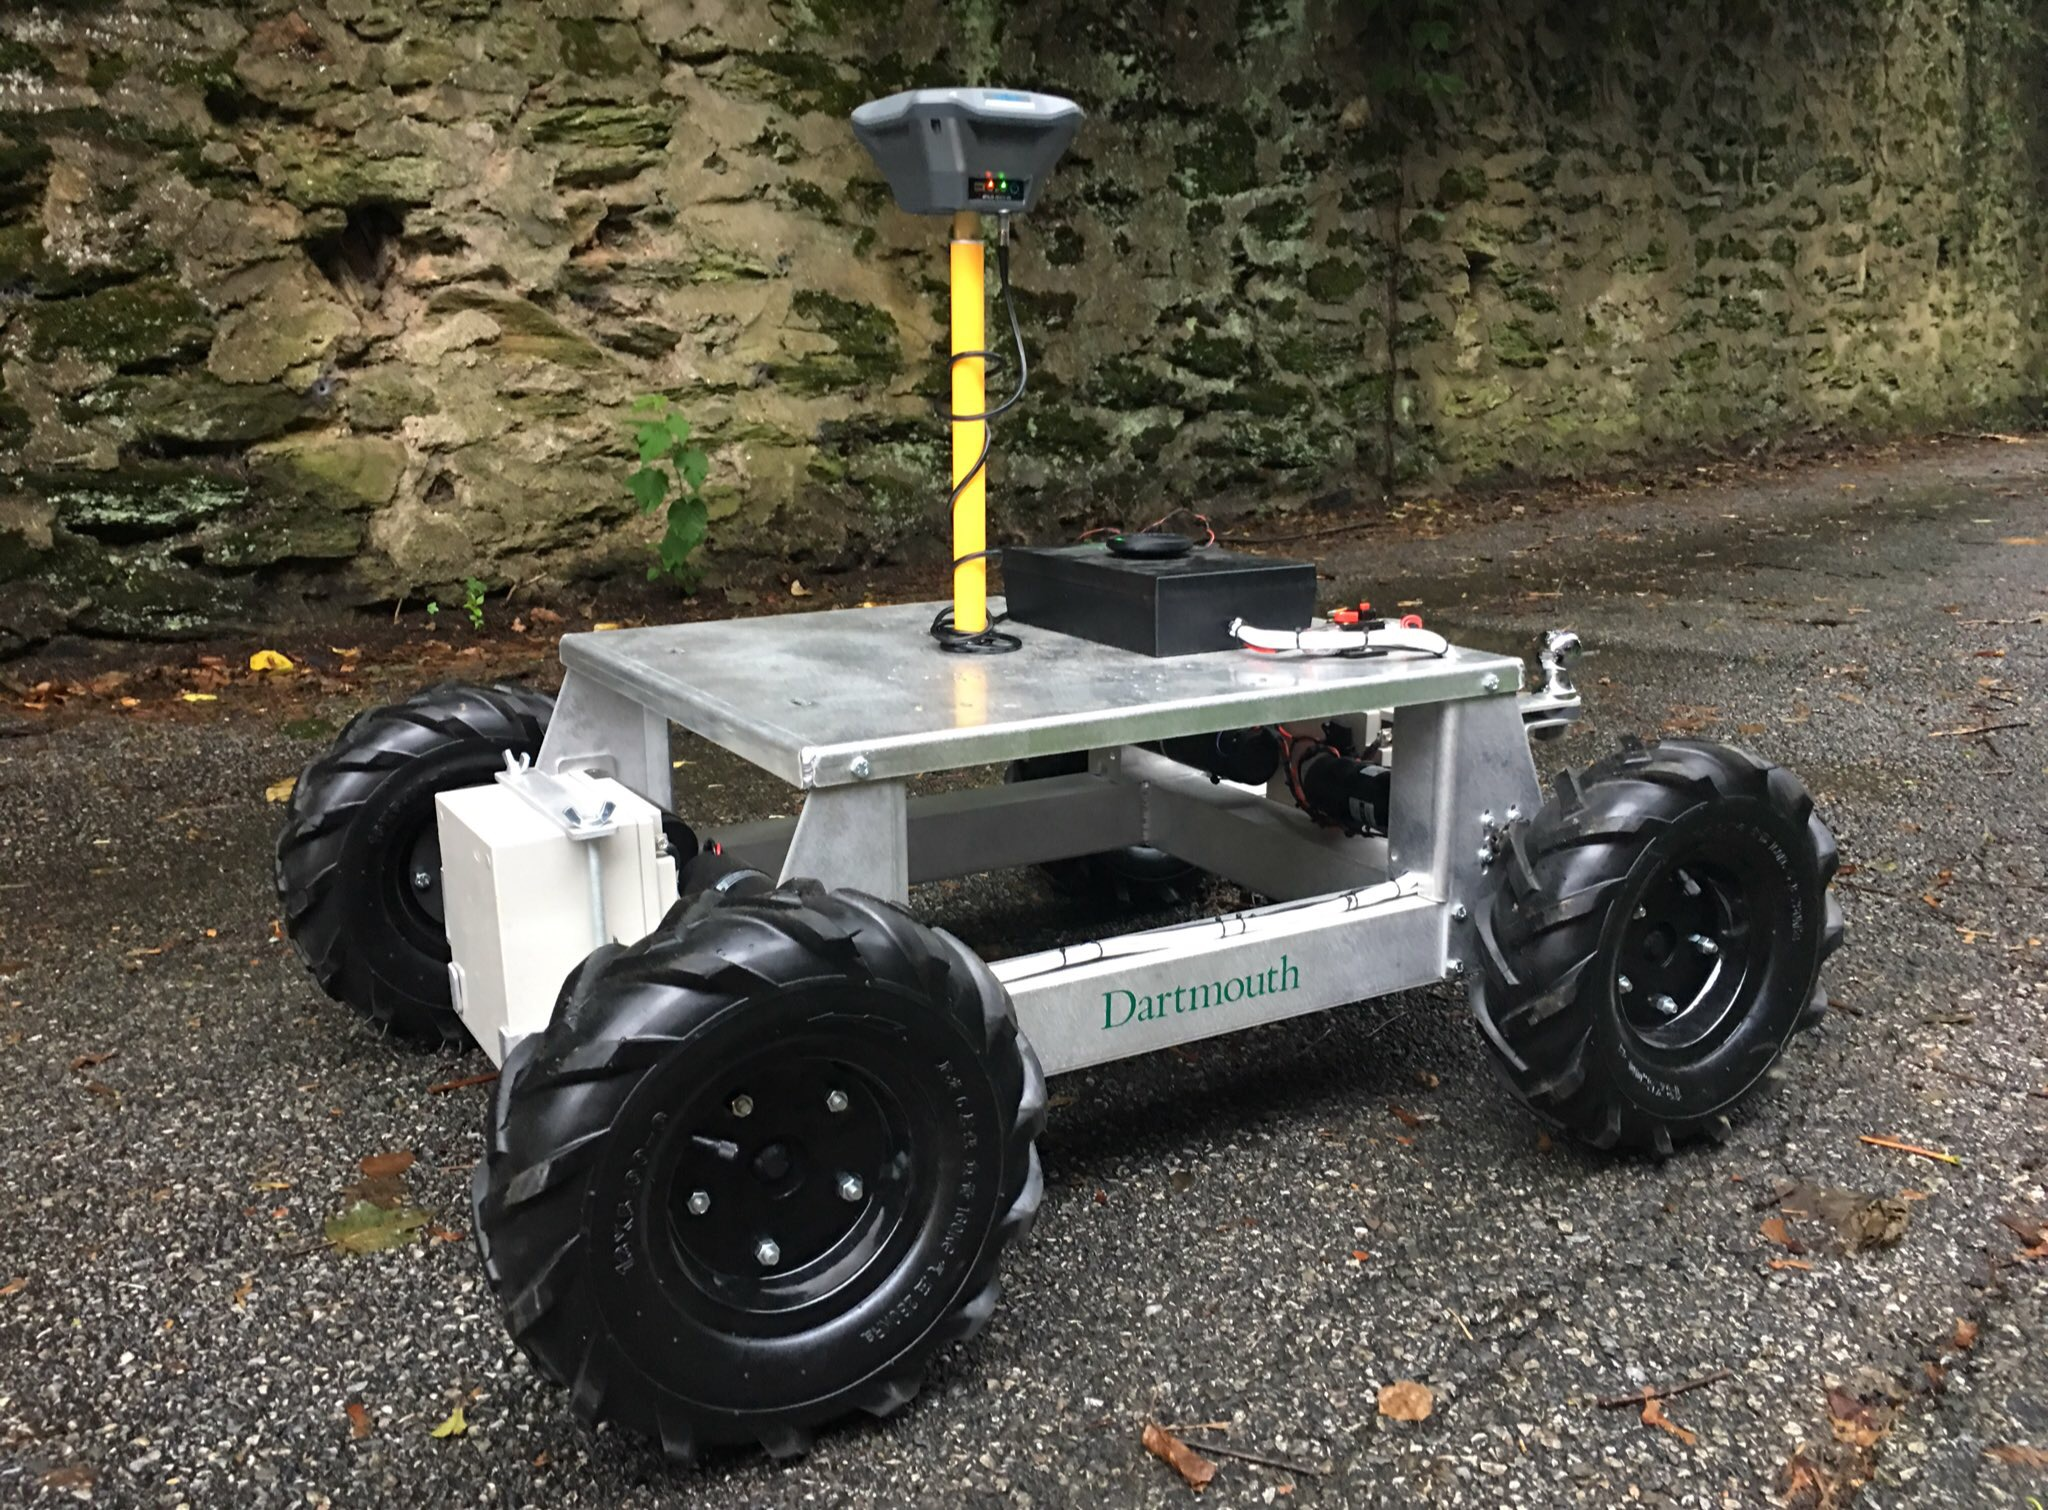
\includegraphics[width=0.4\textwidth]{images/rover.jpeg} }}
    \qquad
    \subfloat[\centering Sub]{{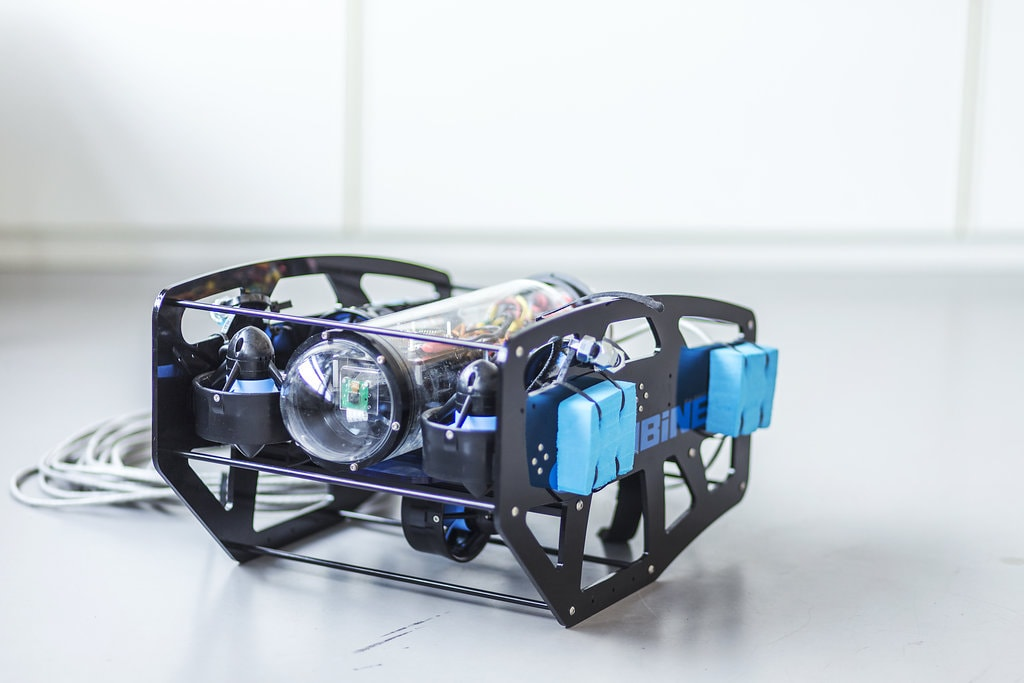
\includegraphics[width=0.4\textwidth]{images/sub.jpeg} }}
\end{figure}

Il progetto fornisce anche del codice specifico per apparati "complementari" ai dispositivi qui sopra descritti. In particolare:

\begin{itemize}
    \item \textbf{AntennaTracker}: che permette di governare apparati che si occupano di ricevere il segnale proveniente dai dispositivi controllati da remoto\cite{antennatracker};
    \item \textbf{Blimp}: un particolare tipo di "pallone" aerostatico dotato di motore\cite{blimp}.
\end{itemize}

\begin{figure}[H]
    \centering
    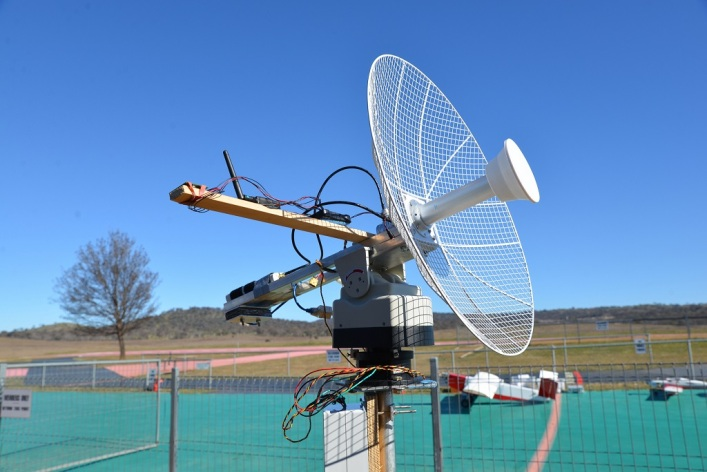
\includegraphics[width=0.8\textwidth]{images/antenna.jpg}
    \caption{AntennaTracker}
\end{figure}
\begin{figure}[H]
    \centering
    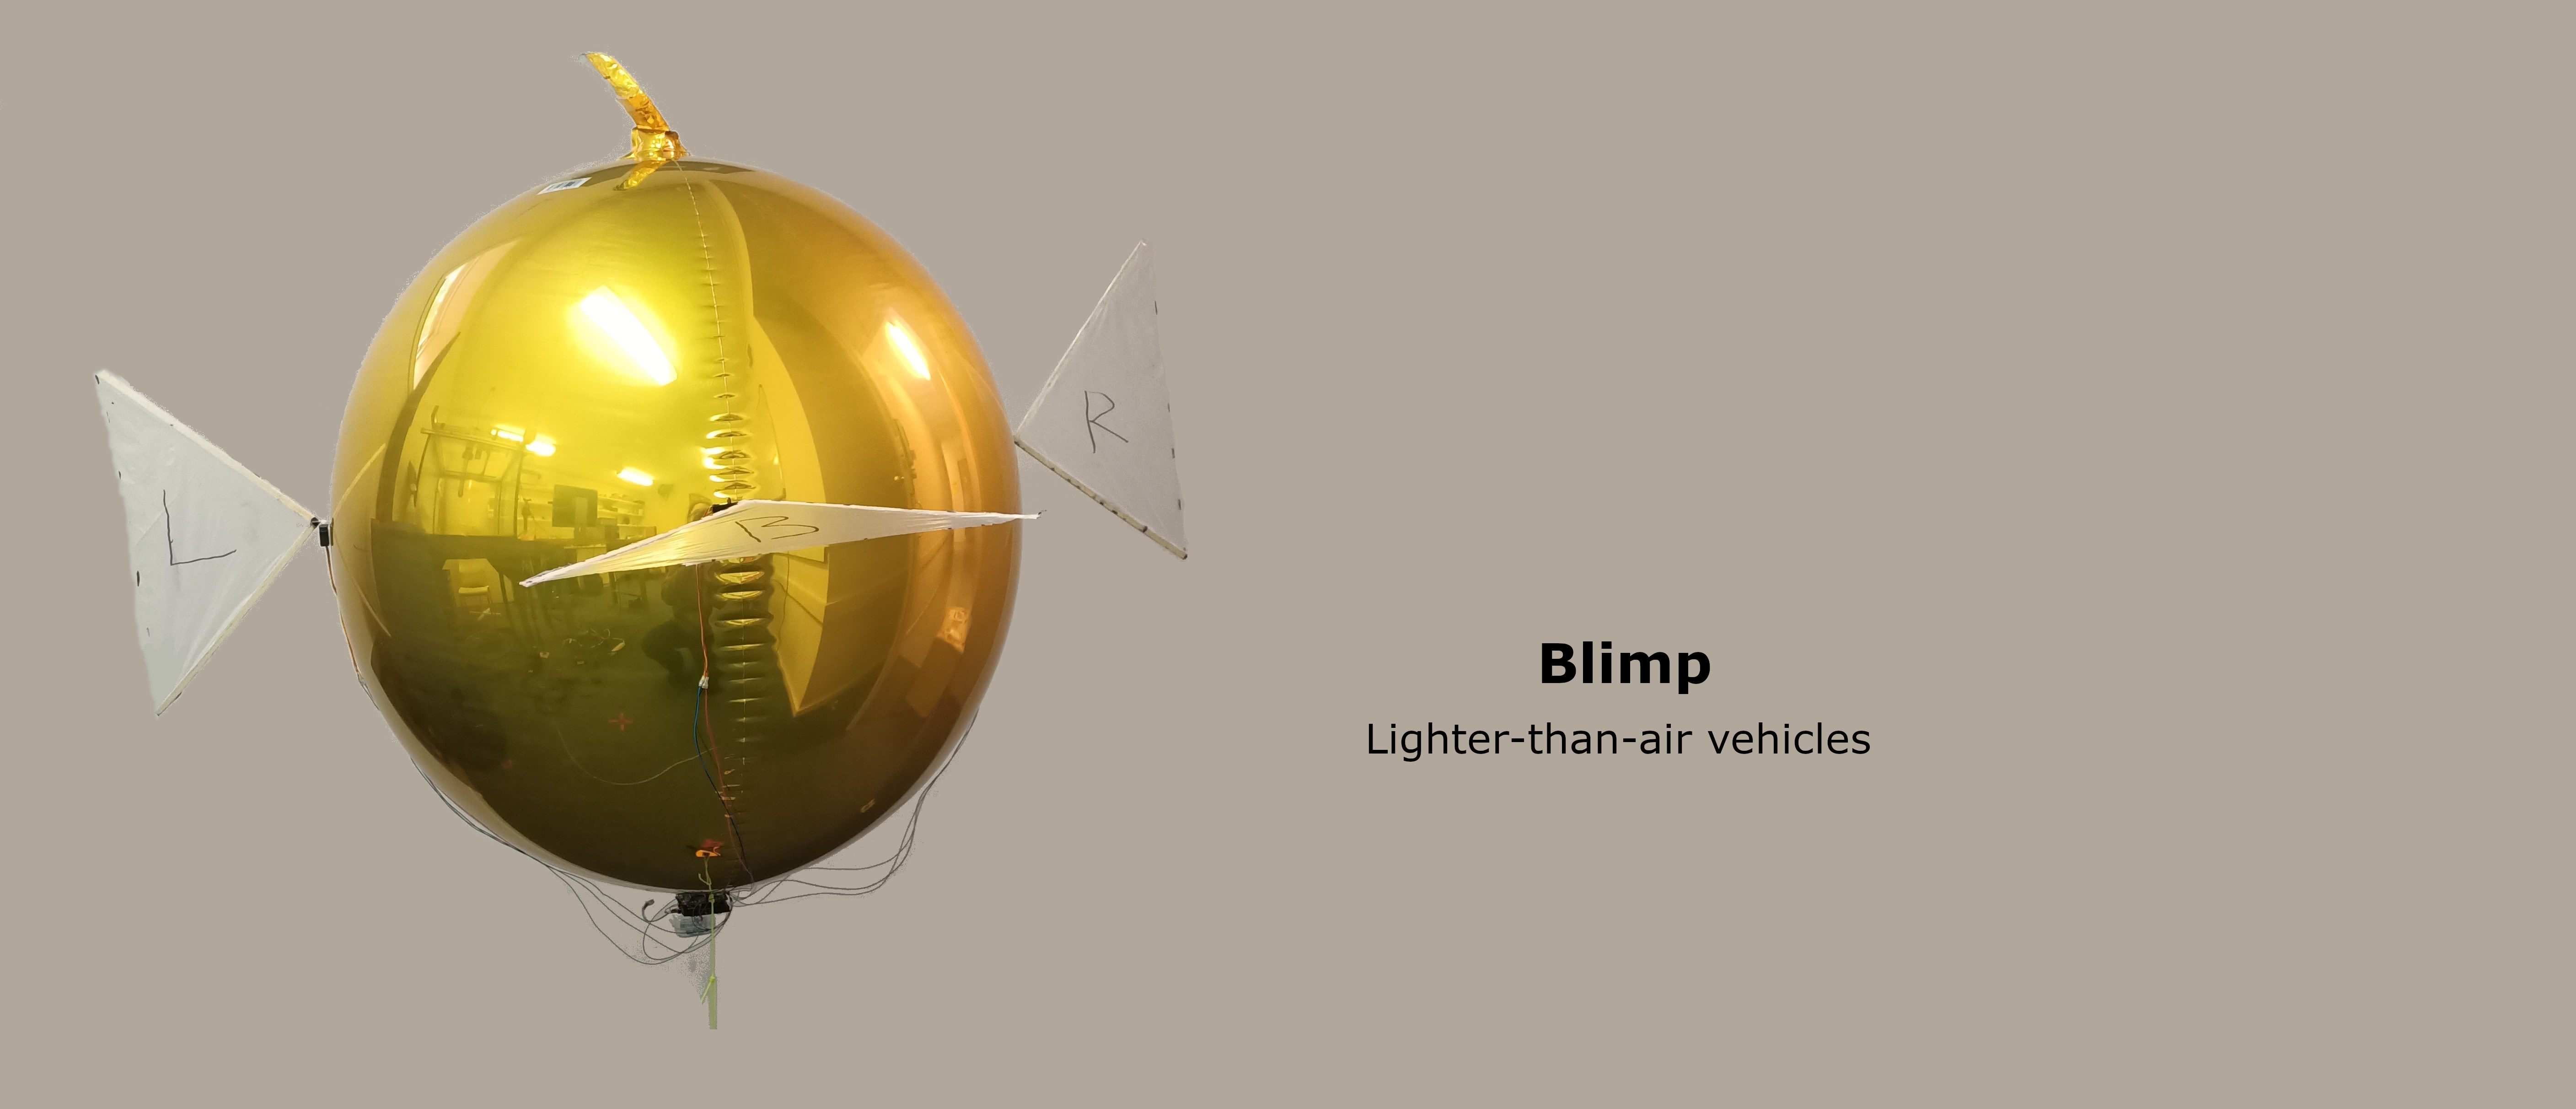
\includegraphics[width=0.8\textwidth]{images/blimp.png}
    \caption{Blimp}
\end{figure}

\subsubsection{SITL - Software in the Loop}
Il progetto ArduPilot mette inoltre a disposizione anche un \textbf{emulatore} che permette il testing di tutte queste varianti della piattaforma \textbf{senza possedere l'hardware adatto} \cite{sitl} e quindi procedere al \textbf{flashing} del firmware. Tale emulatore prende il nome di \textbf{SITL} (\textit{Software In The Loop}) e risulta quindi molto utile quando è necessario svolgere attività di testing preliminari per valutare il comportamento del firmware in use case differenti. Tra l'altro, proprio l'utilizzo di SITL ha permesso la realizzazione di questo lavoro in totale autonomia da hardware specifico. Maggiori informazioni su SITL e sul suo utilizzo saranno proposte in una successiva sottosezione dove verranno presentati ulteriori dettagli sull'architettura software del progetto ArduPilot.

\subsection{ArduPilot: architettura software}
Come menzionato in precedenza, il progetto ArduPilot utilizza il linguaggio di programmazione \textbf{C++}, che è uno di quelli più utilizzati per la programmazione di sistemi embedded in generale poiché \textbf{gira direttamente sull'hardware} senza bisogno di macchine virtuali di sorta (al contrario di Java o di linguaggi interpretati), permettendo di ottenere prestazioni migliori in un contesto in cui proprio le prestazioni rappresentano un requisito fondamentale.

Dal punto di vista della configurazione del progetto, la scelta degli sviluppatori di ArduPilot è ricaduta sul framework \textbf{waf}. Tale framework, scritto in Python, offre un ambiente di build modulare e per quanto possibile agnostico rispetto ai linguaggi di programmazione utilizzati nel progetto col quale lo si vuole usare.

In breve, la documentazione di waf \cite{waf} suggerisce che:

\begin{itemize}
    \item Per utilizzare il framework è necessaria unicamente un'installazione di \textbf{Python};
    \item Waf non definisce un nuovo "linguaggio" (come avviene nel meccanismo dei \textbf{Makefile}) ma si compone di moduli scritti in Python, che permette quindi una maggiore riusabilità delle componenti;
    \item I "target" sono definiti come oggetti python dichiarati in maniera separata dai comandi (definiti invece come funzioni in un file chiamato \texttt{wscript}).
\end{itemize}

Il progetto GitHub della piattaforma ArduPilot contiene il codice sorgente specifico di tutte le tipologie di veicolo, organizzato in directory separate. In particolare:

\begin{itemize}
    \item \texttt{ArduCopter/} contiene il codice sorgente specifico per i veicoli di tipo \textbf{Copter};
    \item \texttt{ArduPlane/} contiene il codice sorgente specifico per i veicoli di tipo \textbf{Plane};
    \item \texttt{ArduSub/} contiene il codice sorgente specifico per i veicoli di tipo \textbf{Sub};
    \item \texttt{Rover/} contiene il codice sorgente specifico per i veicoli di tipo \textbf{Rover};
    \item \texttt{AntennaTracker/} contiene il codice sorgente specifico per i dispositivi che comandano \textbf{antenne di invio/ricezione};
    \item \texttt{Blimp/} contiene il codice sorgente specifico per i veicoli di tipo \textbf{Blimp}, come descritti in precedenza;
\end{itemize}

Inoltre, mediante il comando \texttt{configure} ed il parametro \texttt{-{}-board=} è possibile personalizzare ulteriormente la compilazione del firmware adattandolo ad un \textit{tipo di board} specifico o istruendo il sistema a prepararsi ad essere utilizzato mediante \textbf{SITL}. Quest'ultimo scenario è quello utilizzato nel presente lavoro e si ottiene eseguendo il comando:

\begin{center}
    \texttt{./waf configure -{}-board=sitl}
\end{center}

e, per generare il firmware specifico per un determinato tipo di veicolo (in questo caso quello di elezione è \textbf{Copter}), è necessario eseguire il seguente comando:

\begin{center}
    \texttt{./waf copter}
\end{center}

Per avviare l'emulatore \textbf{SITL} configurato in precedenza è necessario recarsi nella directory del veicolo per cui si è scelto di compilare il firmware (specificato nel comando precedente) (in questo caso, \texttt{ArduCopter/})

\begin{center}
    \texttt{cd ArduCopter/}
\end{center}

e finalmente eseguire l'emulatore mediante il comando

\begin{center}
    \texttt{sim\_vehicle.py}
\end{center}

Nota: il file appena descritto è presente nel percorso \texttt{/Tools/autotest/sim\_vehicle.py} ma non è necessario specificare il suo path assoluto perché durante l'installazione dei prerequisiti di ArduPilot, quest'ultimo viene aggiunto alla \textbf{variabile d'ambiente} \texttt{PATH}.

A questo punto, il veicolo "virtuale" è pronto ad accettare connessioni da una GCS. In particolare, viene aperta la porta \textbf{5760} sull'interfaccia di \textbf{loopback} locale.

È anche possibile modificare il numero di porta utilizzato e l'interfaccia su cui mettersi in ascolto.

\newpage
\printbibliography[title={Riferimenti bibliografici}]
\end{document}